\documentclass{article}
\usepackage[utf8]{inputenc}
\usepackage[english]{babel}
\usepackage[]{amsthm} 
\usepackage[]{amssymb} 
\usepackage{amsmath}
\DeclareMathOperator{\domain}{dom}
\usepackage{graphicx}
\usepackage{hyperref}
\usepackage{comment}
\usepackage[dvipsnames]{xcolor}
\usepackage[thinc]{esdiff}
\usepackage{tcolorbox}
\usepackage{cancel}
\usepackage{graphicx}
\usepackage{float}
\graphicspath{ {./HW2_images/} }
\newtheorem*{theorem}{Theorem}
\newenvironment{solution}
  {\renewcommand\qedsymbol{$\blacksquare$}\begin{proof}[Solution]}
  {\end{proof}}
\DeclareMathOperator{\interior}{int}

\title{Optimization Algorithms: HW2}
\author{Lo Chun, Chou \\ R13922136}
\date\today

\begin{document}
\setlength{\parindent}{0pt}
\maketitle 

\tcbset{
    greenbox/.style={
        colback=SpringGreen!20,
        colframe=SpringGreen!80,
        coltitle=black,
        sharp corners
    },
    bluebox/.style={
        colback=SkyBlue!20,
        colframe=SkyBlue!80,
        coltitle=black,
        sharp corners
    },
    yellowbox/.style={
        colback=yellow!10,
        colframe=yellow!80,
        coltitle=black,
        sharp corners
    }
}

\section*{1}

We're given the following problem:

\begin{align*}
    x_{\star} \in \arg\min_{x \in \Delta_d} f(x), \qquad f(x) = -\sum_{i=1}^n w_i \log \langle a_i, x \rangle
\end{align*}

where:

\begin{enumerate}
    \item 
    \begin{align*}
        x \in \Delta_d = \{ x \in \mathbb{R}^d \mid x[i] \geq 0, \sum_{i=1}^d x[i] = 1 \} \ (\text{probabilit`y simplex})
    \end{align*}
    \item 
    \begin{align*}
        w_i \in \mathbb{R}, \ w_i > 0, \ \sum_{i=1}^n w_i = 1
    \end{align*}
    \item 
    \begin{align*}
        &a_i \in \mathbb{R}^d, \ 
        a_i =
        \begin{bmatrix}
            a_i[1] \\
            a_i[2] \\
            \vdots \\
            a_i[d]
        \end{bmatrix}, \\ 
        &a_i[j] \geq 0 \ \forall i = 1, \dots, n, \ j = 1, \dots, d \\
        &a_i \neq 0 \ \forall i = 1, \dots, n
    \end{align*}
\end{enumerate}

We're asked to show that:

$f$ is $1$-smooth relative to the log-barrier, which is defined as:

\begin{align*}
    h(x) = -\sum_{i=1}^d \log x[i]
\end{align*}

\begin{solution}
%     By lecture slide 4, p.13, we have the definition of relative smoothness:
    
%     \begin{tcolorbox}[bluebox]
%         A function $f$ is $L$-smooth relative to a convex function $h$ for some $L > 0$ if:
%         \begin{align*}
%             f(y) \leq f(x) + \langle \nabla f(x), y - x \rangle + L D_h(y, x)
%         \end{align*}
%     \end{tcolorbox}
% \end{solution}

% Therefore, we need to prove that the following condition holds:

% \begin{align*}
%     -\sum_{i=1}^n w_i \log \langle a_i, y \rangle 
%     \leq -\sum_{i=1}^n w_i \log \langle a_i, x \rangle + \langle \nabla f(x), y - x \rangle + L \{ h(y) - \left[h(x) + \langle \nabla h(x), (y - x) \rangle \right]\}
% \end{align*}

By the following proposition
\footnote{\textit{Relative Smooth Convex Optimization by First-Order Methods, and Applications}, MIT Lecture Notes, available at: \url{https://dspace.mit.edu/bitstream/handle/1721.1/120867/16m1099546.pdf}, accessed: May.~9, 2025, p.~336.}:
\begin{figure}[H]
    \centering
    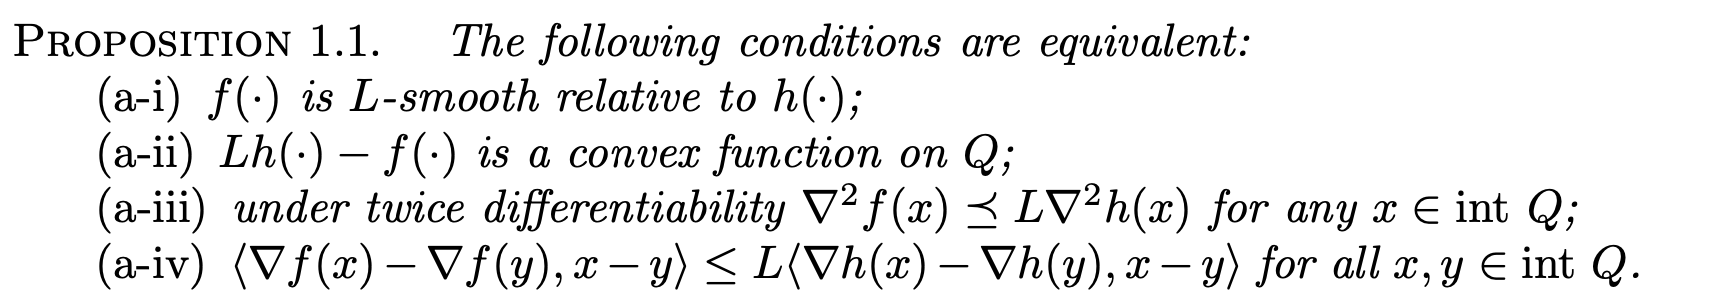
\includegraphics[width = 0.8\textwidth]{proposition_1.1}
\end{figure}
\bigskip

we could prove the required condition (which is (a-i), with $L = 1$) 
by proving its equivalent condition (a-iii, with $L = 1$).
\bigskip

First calculate $\nabla f(x)$:

\begin{align*}
    \nabla f(x) 
    &= \frac{d}{dx} \left( -\sum_{i=1}^n w_i \log \langle a_i, x \rangle \right) \\
    &= -\sum_{i=1}^n w_i \cdot \frac{d}{dx} \left( \log \langle a_i, x \rangle \right) \\
    &= -\sum_{i=1}^n w_i \cdot \left(\frac{a_i}{\langle a_i, x \rangle}\right) \\
    &= -\sum_{i=1}^n w_i \frac{a_i}{\langle a_i, x \rangle}
\end{align*}

Then the Hessian of $f$ is:

\begin{align*}
    \nabla^2 f(x) 
    &= \frac{d}{dx} \left( -\sum_{i=1}^n w_i \frac{a_i}{\langle a_i, x \rangle} \right) \\
    &= -\sum_{i=1}^n w_i \cdot \frac{d}{dx} \left( \frac{a_i}{\langle a_i, x \rangle} \right) \\
    &= -\sum_{i=1}^n w_i \cdot \left( \frac{a_i }{\langle a_i, x \rangle^2} a_i^T\right) \\
\end{align*}

Expanding the expression and writing in another form, we have:

\begin{align*}
    \nabla^2 f(x) 
    &= -\sum_{i=1}^n \frac{w_i}{\langle a_i, x \rangle^2} a_i a_i^T \tag{1}
\end{align*}

Then we shall do the same to $h(x)$

\begin{align*}
    \nabla h(x) 
    &= \frac{d}{dx} \left( -\sum_{i=1}^d \log x[i] \right) \\
    &= 
    \begin{bmatrix}
        -\frac{1}{x[1]} \\
        -\frac{1}{x[2]} \\
        \vdots \\
        -\frac{1}{x[d]}
    \end{bmatrix}
\end{align*}

Then $\nabla^2 h(x)$ is:

\begin{align*}
    \nabla^2 h(x) 
    &= \nabla 
    \begin{bmatrix}
        -\frac{1}{x[1]} \\
        -\frac{1}{x[2]} \\
        \vdots \\
        -\frac{1}{x[d]}
    \end{bmatrix} \\
    &= 
    \begin{bmatrix}
        &\frac{d}{dx[1]} \left( -\frac{1}{x[1]} \right) &\frac{d}{dx[2]} \left( -\frac{1}{x[1]} \right) &\cdots &\frac{d}{dx[d]} \left( -\frac{1}{x[1]} \right) \\
        &\frac{d}{dx[1]} \left( -\frac{1}{x[2]} \right) &\frac{d}{dx[2]} \left( -\frac{1}{x[2]} \right) &\cdots &\frac{d}{dx[d]} \left( -\frac{1}{x[2]} \right) \\
        &\vdots & & \ddots & \vdots \\
        &\frac{d}{dx[1]} \left( -\frac{1}{x[d]} \right) &\frac{d}{dx[2]} \left( -\frac{1}{x[d]} \right) &\cdots &\frac{d}{dx[d]} \left( -\frac{1}{x[d]} \right)
    \end{bmatrix} \\
    &=
    \begin{bmatrix}
        \frac{1}{x[1]^2} & 0 & \cdots & 0 \\
        0 & \frac{1}{x[2]^2} & \cdots & 0 \\
        \vdots & & \ddots & \vdots \\
        0 & 0 & \cdots & \frac{1}{x[d]^2}
    \end{bmatrix} \tag{2}
\end{align*}

Observe $\nabla^2 f(x)$ in $(1)$, since we're given $w_i > 0$, $x \in \Delta_d$, $a_i \neq 0$, 
and with proposition (a-iii) only requires dealing with $\interior \Delta_d$,
we can guarantee $x[i] > 0$, 
so the scalar $\frac{w_i}{\langle a_i, x \rangle^2} > 0$.
\bigskip

Also, we knew that for any $a_i \neq 0$, $a_i a_i^T$ is positive semidefinite,
thus, each term in the summation is positive semidefinite, 
by summing up the $n$ terms and adding a negative sign,
we have $\nabla^2 f(x) \preceq 0$ as follows:

\begin{align*}
    \nabla^2 f(x) 
    = -\sum_{i=1}^n \frac{w_i}{\langle a_i, x \rangle^2} a_i a_i^T \preceq 0
\end{align*}



% We then first show that $\nabla^2 f(x)$ is symmetric, and $\nabla^2 h(x)$ is positive definite,
% in order to use the following generalized Rayleigh quotient to prove that $\nabla^2 f(x) \preceq L \nabla^2 h(x)$:

% \begin{figure}[H]
%     \centering
%     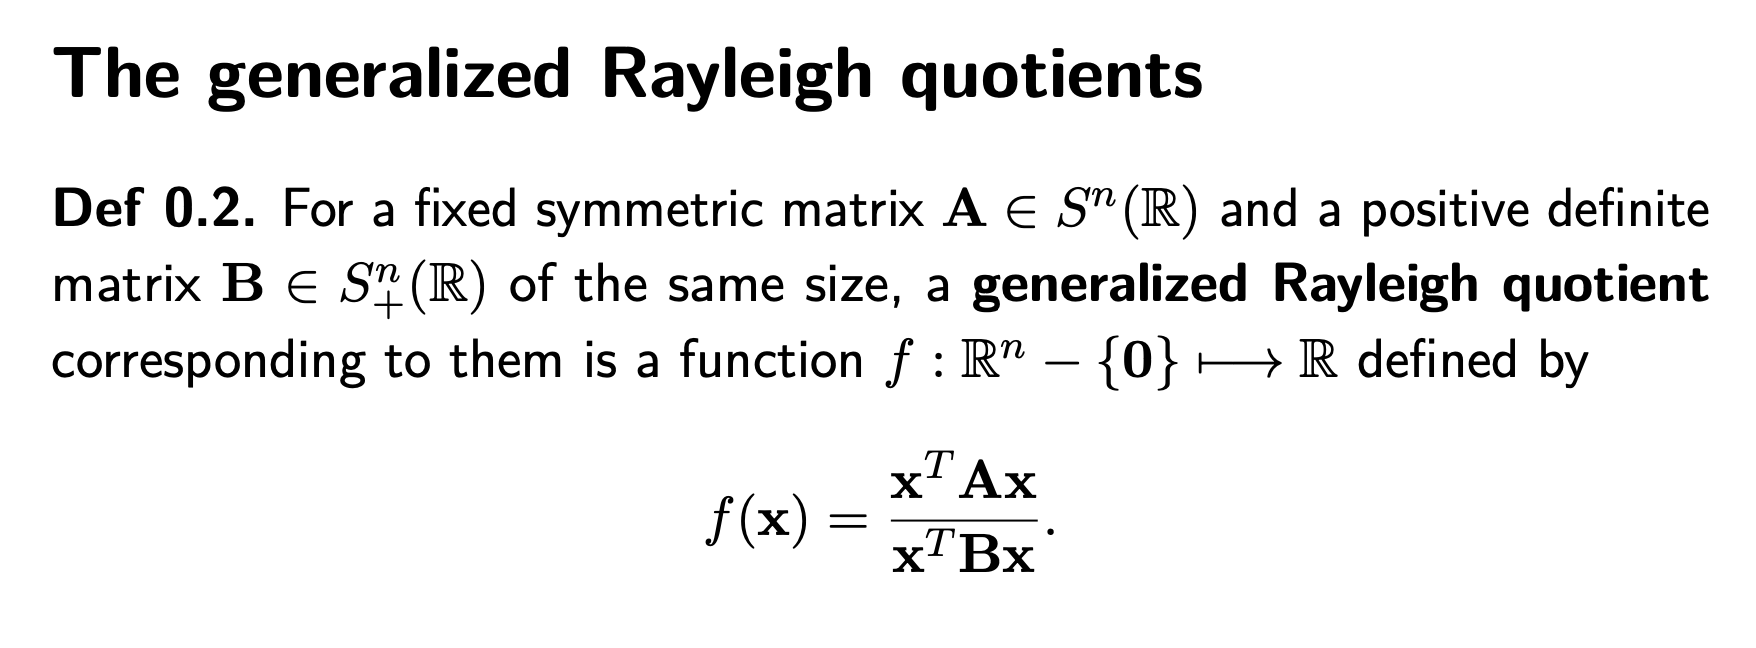
\includegraphics[width = 0.8\textwidth]{generalized_rayleigh_quotients.png}
% \end{figure}

% By our previous calculation, we have:

% \begin{align*}
%     \nabla^2 f(x) = -\sum_{i=1}^n \left( \frac{w_i}{\langle a_i, x \rangle^2} a_i a_i^T\right)
% \end{align*}

% Since $a_i a_i^T$ is symmetric, and multiplying a scalar $\frac{w_i}{\langle a_i, x \rangle^2}$, 
% summing up symmetric matrices also results in a symmetric matrix,
% we have $\nabla^2 f(x)$ is symmetric.
% \bigskip

Then, since $\nabla^2 h(x)$ is a diagonal matrix, and we're given that $x[i] \geq 0$,
same as above, with proposition (a-iii) only requires dealing with $\interior \Delta_d$,
we can guarantee $x[i] > 0$ (so for each $\frac{1}{x[i]}$), and $\nabla^2 h(x)$ is positive definite.
\bigskip

Therefore, we have:

\begin{align*}
    \nabla^2 f(x) \preceq 1 \cdot \nabla^2 h(x) \quad \text{ for any } x \in \interior \Delta_d
\end{align*}

which means that (a-iii) is proved, 
and its equivalent condition (a-i) is also proved, and we have:

\begin{align*}
    f \text{ is } 1\text{-smooth relative to the log-barrier } h
\end{align*}



% Therefore, by letting $A = \nabla^2 f(x)$ and $B = \nabla^2 h(x)$,
% with $z \in \mathbb{R}^d - \{0\}$,
% we define the generalized Rayleigh quotient:

% \begin{align*}
%     R(z) 
%     &= \frac{z^T \nabla^2 f(x) z}{z^T \nabla^2 h(x) z} \\
%     &= \frac{z^T \left( -\sum_{i=1}^n \left( \frac{w_i}{\langle a_i, x \rangle^2} a_i a_i^T\right) \right) z}{-\sum_{i=1}^d \left( \frac{1}{x[i]} z[i]^2\right)} \\
%     &= \frac{\sum_{i=1}^n \left( \frac{w_i}{\langle a_i, x \rangle^2} z^T a_i a_i^T z\right) }{-\sum_{i=1}^d \left( \frac{1}{x[i]} z[i]^2\right)} \\
%     &= \frac{\sum_{i=1}^n \left( \frac{w_i}{\langle a_i, x \rangle^2} \Vert a_i^T z \Vert^2 \right) }{-\sum_{i=1}^d \left( \frac{1}{x[i]} z[i]^2\right)} \\
%     &= \frac{\sum_{i=1}^n \left[ \frac{w_i}{\langle a_i, x \rangle^2} \textcolor{blue}{\left( \sum_{j=1}^d a_i[j] z[j] \right)^2} \right] }{-\sum_{i=1}^d \left( \frac{1}{x[i]} z[i]^2\right)} \\
% \end{align*}

% Using Cauchy-Schwarz inequality in $\mathbb{R}^d$, which is
% \footnote{\textit{Cauchy-Schwarz inequality}, available at: \url{https://en.wikipedia.org/wiki/Cauchy–Schwarz_inequality}, accessed: May.~10, 2025.}:

% \begin{align*}
%     \left( \sum_{i=1}^d u_i v_i \right)^2 \leq \left( \sum_{i=1}^d u_i^2 \right) \left( \sum_{i=1}^d v_i^2 \right)
% \end{align*}

% we have:

% \begin{align*}
%     \left( \sum_{i=1}^d a_i[j] z[j] \right)^2
%     \leq \left( \sum_{i=1}^d a_i[j]^2 \right) \left( \sum_{i=1}^d z[j]^2 \right)
% \end{align*}

% Thus we can bound the previous expression and get:

% \begin{align*}
%     \frac{\sum_{i=1}^n \left[ \frac{w_i}{\langle a_i, x \rangle^2} \textcolor{blue}{\left( \sum_{j=1}^d a_i[j] z[j] \right)^2} \right] }{-\sum_{i=1}^d \left( \frac{1}{x[i]} z[i]^2\right)}
%     \leq \frac{\sum_{i=1}^n \left[ \frac{w_i}{\langle a_i, x \rangle^2} \textcolor{blue}{\left( \sum_{j=1}^d a_i[j]^2 \right) \left( \sum_{j=1}^d z[j]^2 \right)} \right] }{-\sum_{i=1}^d \left( \frac{1}{x[i]} z[i]^2\right)}
% \end{align*}



\end{solution}

\newpage


Denote the Bregman divergence associated with $h$ as $D_h$, i.e.,

\begin{align*}
    D_h(y, x) = h(y) - \left[h(x) + \langle \nabla h(x), (y - x) \rangle \right]
\end{align*}

Consider solving the optimization problem $(1)$ by the following algorithm:

\begin{itemize}
    \item Let $x_1 = 
    \begin{bmatrix}
        \frac{1}{d} \\
        \vdots \\
        \frac{1}{d}
    \end{bmatrix} 
    \in \Delta_d$
    \item For every $t \in \mathbb{N}$, compute:
    \begin{align*}
        x_{t+1} \in \arg\min_{x \in \Delta_d} \left[ \langle \nabla f(x_t), x - x_t \rangle + D_h(x, x_t) \right]
    \end{align*}
\end{itemize}

Note: I use 
$\begin{bmatrix}
    \frac{1}{d} \\
    \vdots \\
    \frac{1}{d}
\end{bmatrix}$ 
to represent the vector $(1/d, \dots, 1/d)$ (which is the notation used in the HW spec) in the following solution.
\section*{2}

Show that for any $x \in \Delta_d$ and $0 \leq \alpha < 1$,

\begin{align*}
    f(x_\alpha) \leq f(x) + \frac{\alpha}{1 - \alpha}, \quad \text{where} \ x_\alpha 
    = (1 - \alpha) x + \alpha 
    \begin{bmatrix}
        \frac{1}{d} \\
        \vdots \\
        \frac{1}{d}
    \end{bmatrix}
\end{align*}

\begin{solution}
From the previous subproblem, we knew that $f$ is $1$-smooth relative to the log-barrier, so we have:

\begin{align*}
    f(y) \leq f(x) + \langle \nabla f(x), y - x \rangle + D_h(y, x) \quad \forall x, y \in \interior \Delta_d
\end{align*}

To bound $f(x_\alpha)$, we first show that $x_\alpha \in \interior \Delta_d$, 
and then let $y = x_\alpha, \ x = x$ so that we would have:

\begin{align*}
    f(x_\alpha) \leq f(x) + \langle \nabla f(x), x_\alpha - x \rangle + D_h(x_\alpha, x)
\end{align*}

By the definition of $x_\alpha$, we knew that it is the convex combination of $x$ and $\begin{bmatrix}
    \frac{1}{d} \\
    \vdots \\
    \frac{1}{d}
\end{bmatrix}$, 
where $x \in \Delta_d$ and $\begin{bmatrix}
    \frac{1}{d} \\
    \vdots \\
    \frac{1}{d}
\end{bmatrix} = x_1 \in \Delta_d$ as stated in the algorithm.
\bigskip
Also, for each element in $x_\alpha$, we have:

\begin{align*}
    x_\alpha[i] = (1 - \alpha) x[i] + \alpha \left( \frac{1}{d} \right) \qquad \forall i = 1, \dots, d
\end{align*}

Since $x[i] \geq 0$ and $\alpha$ is strictly smaller than $1$,
we have $x_\alpha[i] > 0$ for all $i = 1, \dots, d$,
so $x_\alpha \in \interior \Delta_d$.
\bigskip

Then, we have:

\begin{align*}
    f(x_\alpha) \leq f(x) + \langle \nabla f(x), x_\alpha - x \rangle + L D_h(x_\alpha, x)
\end{align*}

To further simplify, we have:

\begin{align*}
    x_\alpha - x 
    = \left[ (1 - \alpha) x + \alpha 
    \begin{bmatrix}
        \frac{1}{d} \\
        \vdots \\
        \frac{1}{d}
    \end{bmatrix}
    \right] - x = \alpha \left[ \begin{bmatrix}
    \frac{1}{d} \\
    \vdots \\
    \frac{1}{d} \end{bmatrix} - x \right]
\end{align*}

So we could expand the following expressions:

\begin{align*}
    \langle \nabla f(x), x_\alpha - x \rangle
    &= \langle -\sum_{i=1}^n w_i \frac{a_i}{\langle a_i, x \rangle}, \alpha \left( \begin{bmatrix}
    \frac{1}{d} \\
    \vdots \\
    \frac{1}{d} \end{bmatrix} - x \right) \rangle \\
    &= - \frac{\alpha}{d} \sum_{i = 1}^n \frac{w_i}{\langle a_i, x \rangle} 
        \left[a_i[1] \cdots a_i[d]\right]
        \begin{bmatrix}
        1 - x[1] \\
        \vdots \\
        1 - x[d]
        \end{bmatrix} \\
    &= - \frac{\alpha}{d} \sum_{i = 1}^n \frac{w_i}{\langle a_i, x \rangle} \left( \sum_{j = 1}^d a_i[j] - \sum_{j = 1}^d a_i[j] x[j] \right) \\
    &= - \frac{\alpha}{d} \sum_{i = 1}^n \frac{w_i}{\sum_{k = 1}^d a_i[k] x[k]} \left( \sum_{j = 1}^d a_i[j] - \sum_{j = 1}^d a_i[j] x[j] \right) \\
    &= - \frac{\alpha}{d} \sum_{i = 1}^n \frac{w_i \sum_{j = 1}^d a_i[j]}{\sum_{k = 1}^d a_i[k] x[k]} + \frac{\alpha}{d} \sum_{i = 1}^n w_i \\
    &= \frac{\alpha}{d} \left( 1 - \sum_{i = 1}^n w_i \sum_{j = 1}^d \frac{a_i[j]}{a_i[j] x[j]} \right) \\
    &= \frac{\alpha}{d} \left( 1 - \sum_{i = 1}^n w_i \sum_{j = 1}^d \frac{1}{x[j]} \right)
    \tag{1}
\end{align*}

By the definition of $D_h$, we have:

\begin{align*}
    D_h(x_\alpha, x) 
    &= h(x_\alpha) - \left(h(x) + \langle \textcolor{Green}{\nabla h(x)}, \textcolor{blue}{(x_\alpha - x)} \rangle \right) \\
    &= h(x_\alpha) - \left(h(x) + \langle
        \textcolor{Green}{\begin{bmatrix}
        -\frac{1}{x[1]} \\
        -\frac{1}{x[2]} \\
        \vdots \\
        -\frac{1}{x[d]}
        \end{bmatrix}}, 
    \textcolor{blue}{\alpha \left( \begin{bmatrix}
    \frac{1}{d} \\
    \vdots \\
    \frac{1}{d} \end{bmatrix} - x \right) \rangle} \right) \\
    &= -\sum_{i=1}^d \log x_\alpha[i] - \left( -\sum_{i=1}^d \log x[i] + \langle 
    \begin{bmatrix}
        -\frac{1}{x[1]} \\
        -\frac{1}{x[2]} \\
        \vdots \\
        -\frac{1}{x[d]}
    \end{bmatrix}, \alpha \left( \begin{bmatrix}
        \frac{1}{d} \\
        \vdots \\
        \frac{1}{d}
    \end{bmatrix} - x \right) \rangle \right) \\
    &= -\sum_{i=1}^d \log x_\alpha[i] + \sum_{i=1}^d \log x[i] + \alpha [-\frac{1}{x[1]} \cdots -\frac{1}{x[d]}]
    \begin{bmatrix}
        \frac{1 - dx[1]}{d} \\
        \vdots \\
        \frac{1 - dx[d]}{d}
    \end{bmatrix} \\
    &= \sum_{i = 1}^d (\log x[i] - \log x_\alpha[i]) - \sum_{i = 1}^d \frac{\alpha}{d x[i]} + \alpha d \\
    \tag{2}
\end{align*}

Combining (1) and (2), we have:

\begin{align*}
    &\langle \nabla f(x), x_\alpha - x \rangle + D_h(x_\alpha, x) \\
    &= \frac{\alpha}{d} \left( 1 - \sum_{i = 1}^n w_i \sum_{j = 1}^d \frac{1}{x[j]} \right)
        + \sum_{i = 1}^d (\log x[i] - \log x_\alpha[i]) - \sum_{i = 1}^d \frac{\alpha}{d x[i]} + \alpha d \\
    &= 
\end{align*}






\end{solution}

\end{document}